\documentclass[12pt,a4paper]{article}
\usepackage{amsmath}
\usepackage{amssymb}
\usepackage{braket}
\usepackage{graphicx}
\usepackage{footnote}
\usepackage{titlesec}
\usepackage{subfig}
\usepackage{float}
\usepackage{color}   %May be necessary if you want to color links
\usepackage{hyperref}
\hypersetup{
    colorlinks=true, %set true if you want colored links
    linktoc=all,     %set to all if you want both sections and subsections linked
    linkcolor=blue,  %choose some color if you want links to stand out
}
\setcounter{secnumdepth}{4}

\makesavenoteenv{page}

\begin{document}
\title{Black Holes}
\date{}
\maketitle
\small{Name: Vinay Vikramaditya}\\

\small{Sr No: 14416}\\

\newpage
\tableofcontents
\newpage



\section{Kruskal-Szekeres Coordinates}

Let's look at radial light rays given by $ds^{2}=0$ with $d\theta=0$ and $d\phi=0$. This gives 
$$
d t=\pm \frac{1}{1-\frac{r_{\mathrm{S}}}{r}} d r=\pm \frac{r}{r-r_{\mathrm{S}}} d r
$$
The $\pm$ indicate if ray if outgoing or incoming. Far away slopes are $\pm 1$ as expected but as $r \rightarrow r_{S}$, slope $\rightarrow 0$ as shown in Fig 1.
\begin{figure}[H]
  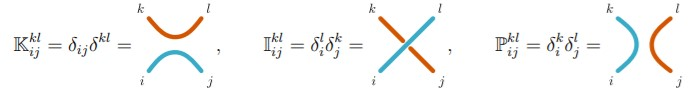
\includegraphics[width=\linewidth]{1.jpg}
  \caption{Light cone variation}
  \label{fig:1}
\end{figure}

We want to make a change of variables. To look at what change of variables is needed we write
$$
\begin{aligned}
d s^{2} &=-\left(1-\frac{r_{\mathrm{S}}}{r}\right)\left(d t^{2}-\frac{1}{\left(1-\frac{r_{\mathrm{S}}}{r}\right)^{2}} d r^{2}\right)+r^{2} d \Omega^{2} \\
&=-\left(\frac{r-r_{\mathrm{S}}}{r}\right)\left(d t+\frac{r}{r-r_{\mathrm{S}}} d r\right)\left(d t-\frac{r}{r-r_{\mathrm{S}}} d r\right)+r^{2} d \Omega^{2}
\end{aligned}
$$
Defining $d \bar{t} \equiv d t+\frac{r_{\mathrm{S}}}{r-r_{\mathrm{S}}} d r$, we get
$$
d s^{2} =-\left(\frac{r-r_{\mathrm{S}}}{r}\right)(d \bar{t}+d r)\left(d \bar{t}-\frac{r+r_{\mathrm{S}}}{r-r_{\mathrm{S}}} d r\right)+r^{2} d \Omega^{2}
$$
For radial light rays, we get for incoming equation to be $d \bar{t}+d r=0$ and outgoing equation to be $d \bar{t}=\frac{r+r_{\mathrm{S}}}{r-r_{\mathrm{S}}} d r$. We see that in all cases incoming slope $=-1$ and outgoing slope is positive for $r>r_{\mathrm{S}}$ and negative for $r<r_{\mathrm{S}}$ as shown in Fig 2. Since both incoming and outgoing light rays are towards the singularity for $r<r_{\mathrm{S}}$ and all material particles can move only inside the cone, nothing can escapethe event horizon.
\begin{figure}[H]
  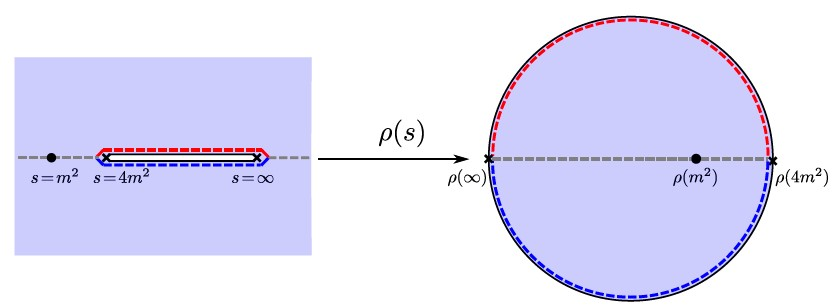
\includegraphics[width=\linewidth]{2.jpg}
  \caption{Light cone variation}
  \label{fig:2}
\end{figure}
A preffered set of coordinates would be that which would have both incoming and outgoing rays to be at $\pm 1$. We start out with change of variables
$d p=d t+\frac{r}{r-r_{\mathrm{S}}} d r$ and $d q=d t-\frac{r}{r-r_{\mathrm{S}}} d r$. Then
$$
d s^{2}=-\left(\frac{r-r_{\mathrm{S}}}{r}\right) d p d q+r^{2} d \Omega^{2}
$$
$r$ is to be regarded as a function of $p$ and $q$. We have $d(p+q)=2 d t$ and $d(p-q)=\frac{2 r}{r-r_{\mathrm{S}}} d r=2\left(1+\frac{r_{\mathrm{S}}}{r-r_{\mathrm{S}}}\right) d r \Rightarrow p+q=2 t$ and $p-q=2 r+2 r_{\mathrm{S}} \log \frac{\left|r-r_{\mathrm{S}}\right|}{r_{\mathrm{S}}}$. The logarithm suggests we write
$$e^{-\frac{p-q}{2r_{\mathrm{S}}}}=e^{-\frac{r}{r_{\mathrm{S}}}} \frac{r_{\mathrm{S}}}{r-r_{\mathrm{S}}}sign(r-r_{\mathrm{S}})$$
We do a change of coordinates $P=e^{p / 2 r_{\mathrm{S}}}$ and $Q=-e^{-q / 2 r_{\mathrm{S}}}$ to get
$$
d s^{2}=-\frac{4 r_{\mathrm{S}}^{3}}{r} e^{-r / r_{\mathrm{S}}} \operatorname{sign}\left(r-r_{\mathrm{S}}\right) d P d Q+r^{2} d \Omega^{2}
$$
To get in the form in which radial rays move at $\pm 1$
$$
d s^{2}=-\frac{4 r_{\mathrm{S}}^{3}}{r} e^{-r / r_{\mathrm{S}}}\left(d V^{2}-d U^{2}\right)+r^{2} d \Omega^{2}
$$
we have to require $d V^{2}-d U^{2}=\operatorname{sign}\left(r-r_{\mathrm{S}}\right) d P d Q$. We see singularity at $r=0$ but not at $r=r_{\mathrm{S}}$. For this to happen, we must define $r>r_{\mathrm{S}}$, we have $V=\frac{1}{2}(P+Q), U=\frac{1}{2}(P-Q)$, and for $r<r_{\mathrm{S}}$ we have $V=\frac{1}{2}(P-Q), U=\frac{1}{2}(P+Q)$. We now get 
$$
\begin{aligned}
V^{2}-U^{2} &=\operatorname{sign}\left(r-r_{\mathrm{S}}\right) P Q=-\operatorname{sign}\left(r-r_{\mathrm{S}}\right) e^{(p-q) / 2 r_{\mathrm{S}}} \\
&=-\operatorname{sign}\left(r-r_{\mathrm{S}}\right)\left(\left|r-r_{\mathrm{S}}\right| / r_{\mathrm{S}}\right) e^{r / r_{\mathrm{S}}}=\left(1-\frac{r}{r_{\mathrm{S}}}\right) e^{r / r_{\mathrm{S}}}
\end{aligned}
$$
Now for $r>r_{\mathrm{S}}, \frac{V}{U}=\frac{P+Q}{P-Q}=\frac{e^{(p+q) / 2 r_{\mathrm{S}}}-1}{e^{(p+q) / 2 r_{\mathrm{S}}}+1}=\tanh \frac{t}{2 r_{\mathrm{S}}}$, while for $r>r_{\mathrm{S}}, \frac{V}{U}=\frac{P-Q}{P+Q}=\frac{e^{(p+q) / 2 r_{\mathrm{S}}}+1}{e^{(p+q) / 2 r_{\mathrm{S}}}-1}=\coth \frac{t}{2 r_{\mathrm{S}}}$. Now using $V^{2}-U^{2}=\left(1-\frac{r}{r_{\mathrm{S}}}\right) e^{r / r_{\mathrm{S}}}$, and the given values of $\frac{V}{U}$ we get 
$$
V=\left(\frac{r}{r_{\mathrm{S}}}-1\right)^{1 / 2} e^{r / 2 r_{\mathrm{S}}} \sinh \left(\frac{t}{2 r_{\mathrm{S}}}\right), \quad U=\left(\frac{r}{r_{\mathrm{S}}}-1\right)^{1 / 2} e^{r / 2 r_{\mathrm{S}}} \cosh \left(\frac{t}{2 r_{\mathrm{S}}}\right)
$$
for outside the horizon and 
$$
V=\left(1-\frac{r}{r_{\mathrm{S}}}\right)^{1 / 2} e^{r / 2 r_{\mathrm{S}}} \cosh \left(\frac{t}{2 r_{\mathrm{S}}}\right), \quad U=\left(1-\frac{r}{r_{\mathrm{S}}}\right)^{1 / 2} e^{r / 2 r_{\mathrm{S}}} \sinh \left(\frac{t}{2 r_{\mathrm{S}}}\right)
$$
for inside the horizon.
\subsection{Kruskal-Szekeres Diagram}
We need to make a plot of spacetime in $V-U$ coordinates. We can use the step function to write
$$
\frac{V}{U}=\Theta\left(r-r_{\mathrm{S}}\right) \tanh \frac{t}{2 r_{\mathrm{S}}}+\Theta\left(r_{\mathrm{S}}-r\right) \operatorname{coth} \frac{t}{2 r_{\mathrm{s}}}=\frac{dV}{dU}
$$
\begin{figure}[H]
    \centering
    \subfloat[\centering Lines of constant $t$ and $r$]{{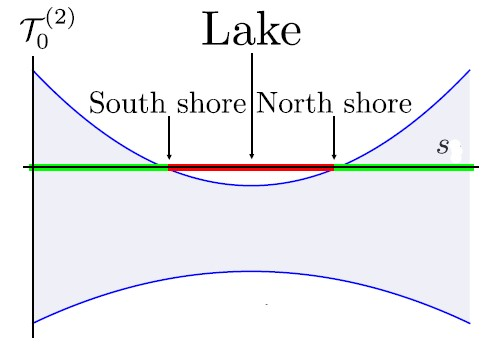
\includegraphics[width=6cm]{3.jpg} }}
    \qquad
    \subfloat[\centering Escape and Gravitational time dilation]{{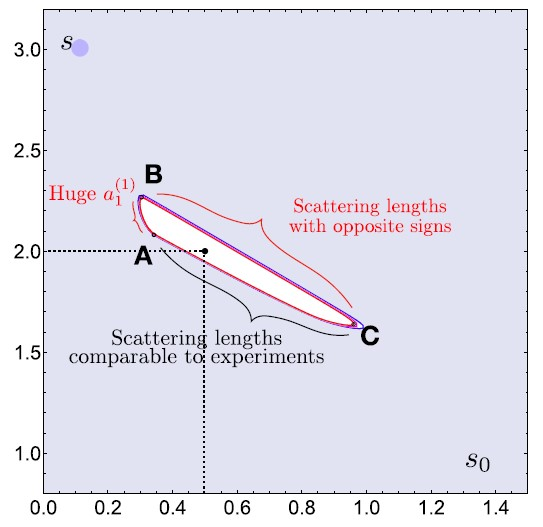
\includegraphics[width=6cm]{4.jpg} }}
    \caption{Kruskal-Szekeres diagram}
    \label{fig:example}
\end{figure}
Lines of constant $t$ correspond to straight lines with constant slope. Also since $V^{2}-U^{2}=\left(1-\frac{r}{r_{\mathrm{S}}}\right) e^{r / r_\mathrm{S}}$, lines of constant $r$ are hyberbolae. They are vertically oriented for $r>r_{\mathrm{S}}$ and horizontally oriented for $r<r_{\mathrm{S}}$. For $r=0$, the hyperbola is $V=+\sqrt{U^{2}+1}$. For $r=r_{\mathrm{S}}=2M$, the hyperbole degenerate to two straight lines $V=\pm U$ and hence at the horizon, vertically oriented hyperbolas transition into horizontally oriented hyperbolas. As $tanh(0)=0$, $tanh(\infty)=1$, $coth(\infty)=1$ and $coth(0)=\infty$. As we approach the horizon, $t$ increases, reaching $\infty$ when we reach the horizon, and after passing it, $t$ decreases from $\infty$. We also make the following observations:\\ 
1. Since for material particles, any trajectory inside the cone is allowed and lightcone has slope $\pm 1$. So, at any point inside the horizon escape is possible but not from inside it in which case all trajectories end at singularity $r=0$.\\
2. The infalling observer sends out signals at regular intervals, and from the figure we see that it reaches a stationery observer at $r$ at ever increasing intervals. This signifies a red-shift/gravitational time dilation.


\section{Penrose Diagrams}
We add one more demand of having range of coordiantes to be finite along with $45^{\circ}$ light rays. We first do this for Minkowski space for simplicity. Minkowski spacetime has $d s^{2}=-d t^{2}+$ $d r^{2}+r^{2} d \Omega^{2}$. Going to light cone coordinates $p=t+r, q=t-r$ so that $d s^{2}=-d p d q+r^{2} d \Omega^{2}$. $t \in (-\infty,\infty)$ and $r \in (0,\infty)$. So $p-q=2 r>0$. $p,q \in (-\infty,\infty)$. We can now use $\tan$ to compactify this as follows: $p=\tan P, q=\tan Q$ and $P, Q\in \left(-\frac{\pi}{2}, \frac{\pi}{2}\right)$. Also $p>q \Rightarrow P>Q$. So, spacetime consists of a triangle bounded by the three straight lines $P=\pi / 2, Q=-\pi / 2$, and $P=Q$. We rotate back using $T=P+Q, R=P-Q$ and spacetime is represented by a triangle bounded by the three straight lines $T=\pi-R, T=-\pi+R$ and $R=0$. \\
To summarise, the overall transformation is just $t\pm r \rightarrow \tan(\frac{T\pm R}{2})$ i.e compactifying light cone coordinates, which gave us
$$
\begin{aligned}
d s^{2} &=-d t^{2}+d r^{2}+r^{2} d \Omega_{d-2}^{2} \\
&=-d p d q+\frac{1}{4}(p-q)^{2} d \Omega_{d-2}^{2} \\
&=\frac{1}{4 \cos ^{2} P \cos ^{2} Q}\left(-d T^{2}+d R^{2}+R^{2} d \Omega_{d-2}^{2}\right)\\
&=\frac{1}{4 \cos ^{2} (\frac{T+R}{2}) \cos ^{2} (\frac{T-R}{2})}\left(-d T^{2}+d R^{2}+R^{2} d \Omega_{d-2}^{2}\right)
\end{aligned}
$$
\begin{figure}[H]
    \centering
    \subfloat[\centering Minkowski]{{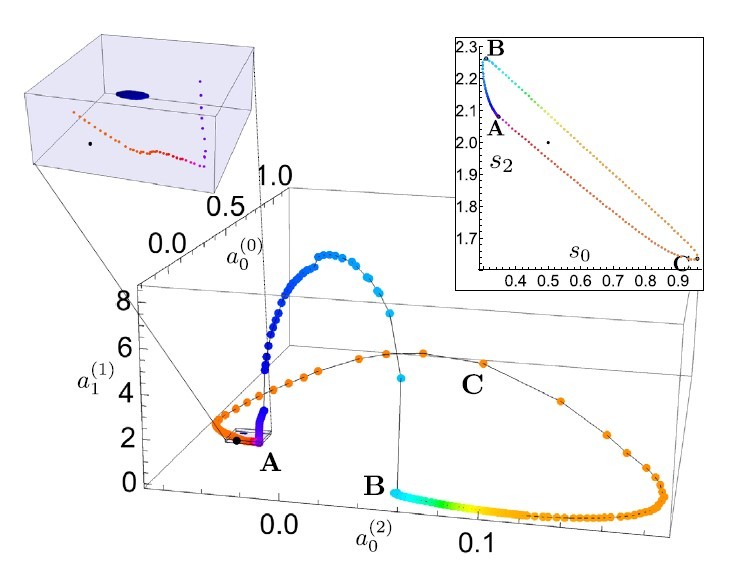
\includegraphics[width=4cm]{5.jpg} }}
    \qquad
    \subfloat[\centering Schwarschild]{{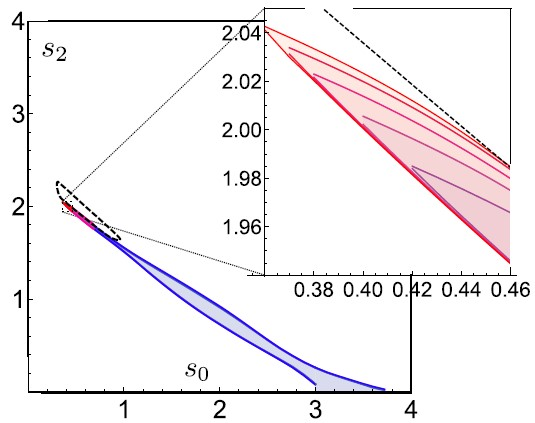
\includegraphics[width=8cm]{6.jpg} }}
    \caption{Penrose diagrams}
    \label{fig:example}
\end{figure}
To get the Penrose diagram for a black hole we take $d s^{2}=-\frac{4 r_{\mathrm{S}}^{3}}{r} e^{-r / r_{\mathrm{S}}}\left(d V^{2}-d U^{2}\right)+r^{2} d \Omega^{2}$ and apply $V\pm U \rightarrow \tan(\frac{T\pm R}{2})$ to obtain 
$$
d s^{2}=\frac{r_{\mathrm{S}}^{3}}{r} \frac{e^{\frac{r}{r_{\mathrm{S}}}}\left(-dT^{2}+dR^{2}\right)}{\cos ^{2}(\frac{T+R}{2}) \cos ^{2}(\frac{T-R}{2})}+r^{2}\left(d \theta^{2}+\sin ^{2} \theta d \phi^{2}\right)
$$
where $r=r(T,R)$ is a solution to the equation 
$$
\left(1-\frac{r}{r_{\mathrm{S}}}\right) e^{\frac{r}{r_{\mathrm{S}}}}=\tan\left(\frac{T+R}{2}\right) \tan\left(\frac{T-R}{2}\right)
$$


\section{Charged Black Hole - Reissner Nordstrom Solution}
We have the same form of spherically symmetric metric given by 
$$d s^{2}=-A(r) d t^{2}+B(r) d r^{2}+r^{2} d \Omega^{2}$$
 $A(r)$ and $B(r)$ which are to be calculated by solving Einstein's equation and also the Maxwell's equation (in its covariant form) $D_{\mu} F^{\mu \nu}=\frac{1}{\sqrt{-g}} \partial_{\mu}\left(\sqrt{-g} F^{\mu \nu}\right)=0 .$ \\
Since we have a spherically symmetric system, electric field has only a radial component $E=F_{0 r}=-F_{r 0}$. And since metric is diagonal, we can write $$F^{0 r}=g^{00} g^{r r} F_{0 r}=\frac{E}{A B}$$
The determinant of the metric is $g=-A B r^{4} \sin ^{2} \theta$ which is independent of $t$. Maxwell's equation gives $\partial_{0}\left(r^{2} E / \sqrt{A B}\right)=0$ which just gives us the expected fact that $E$ is constant over time and thus Maxwell's equations reduce to $\partial_{r}\left(r^{2} E / \sqrt{A B}\right)=0$, with the solution
$$
E=\frac{Q \sqrt{A B}}{r^{2}}
$$
The overall factor in the way electric charge $Q$ is defined is fixed by demanding $E(r) \rightarrow Q / r^{2}$ as $r \rightarrow \infty$ where $A(r) \rightarrow 1, B(r) \rightarrow 1$ since far away from source space is asymtotically flat as energy density of EM field dies off rapidly. Since only $F_{0 r}=-F_{r 0}$ are nonzero components of $F_{\mu \nu}$, $\varepsilon^{\rho \lambda \mu \nu} D_{\lambda} F_{\mu \nu}=$ 0 is automatically satisfied. Now to move towards the Einstein's equations by first writing down the energy momentum tensor for EM field $T_{\mu \nu}=F_{\mu \lambda} F_{\nu}^{\lambda}-\frac{1}{4} g_{\mu \nu} F_{\sigma \rho} F^{\sigma \rho} .$ which is traceless since
$$T=g^{\mu \nu}T_{\mu \nu}=F_{\mu \lambda} F^{\mu \lambda}-\frac{1}{4} \delta^{\mu}_{\mu} F_{\sigma \rho} F^{\sigma \rho}=0$$
So we can now use $R_{\mu \nu}-\frac{1}{2}g_{\mu \nu}R=8 \pi G T_{\mu \nu}$ and use a trace on both sides to get $-R=8 \pi GT=0$ since EM energy momentum tensor is traceless. So we have $R_{\mu \nu}=8 \pi G T_{\mu \nu}$. Additionally we borrow from the Schwarschild case the Ricci tensor components for the spherically symmetric metric at hand
$$
\begin{array}{l}
R_{0 0}=\frac{A^{\prime \prime}}{2 B}+\frac{A^{\prime}}{r B}-\frac{A^{\prime}}{4 B}\left(\frac{A^{\prime}}{A}+\frac{B^{\prime}}{B}\right) \\
R_{r r}=-\frac{A^{\prime \prime}}{2 A}+\frac{B^{\prime}}{r B}+\frac{A^{\prime}}{4 A}\left(\frac{A^{\prime}}{A}+\frac{B^{\prime}}{B}\right) \\
R_{\theta \theta}=1-\frac{1}{B}-\frac{r}{2 B}\left(\frac{A^{\prime}}{A}-\frac{B^{\prime}}{B}\right)
\end{array}
$$
and a useful combination of these
$$
\frac{R_{00}}{A}+\frac{R_{r r}}{B}=\frac{1}{r B}\left(\frac{A^{\prime}}{A}+\frac{B^{\prime}}{B}\right)
$$
We need to calculate $T_{00}$ and $T_{r r}$.
$$T_{00}=F_{0 \lambda} F_{0}^{\;\lambda}-\frac{1}{4} g_{00} F_{\sigma \rho} F^{\sigma \rho}$$
Using $E=F_{0 r}=-F_{r 0}$ and the fact that metric is diagonal, 
$$T_{00}=g^{r r} F_{0 r} F_{0 r}-\frac{1}{4} g_{00}\left(2 F_{0 r} F_{0 r}\right) g^{00} g^{r r}=\frac{E^{2}}{B}+\frac{1}{4}\left(\frac{-2 E^{2}}{B}\right)=\frac{E^{2}}{2 B}$$
Similarily with 
$$T_{r r}=F_{r \lambda} F_{r}^{\;\lambda}-\frac{1}{4} g_{r r} F_{\sigma \rho} F^{\sigma \rho}$$
$$T_{r r}=g^{0 0} F_{r 0} F_{r 0}-\frac{1}{4} g_{r r}\left(2 F_{r 0} F_{r 0}\right) g^{00} g^{r r}=-\frac{E^{2}}{A}+\frac{1}{4}\left(\frac{2 E^{2}}{A}\right)=-\frac{E^{2}}{2 A}$$
So, we have 
$$
\frac{R_{00}}{A}+\frac{R_{r r}}{B}=\frac{1}{r B}\left(\frac{A^{\prime}}{A}+\frac{B^{\prime}}{B}\right)=8\pi G \left(\frac{T_{00}}{A}+\frac{T_{r r}}{B}\right)=0
$$
which is just like in Schwarschild case. So that $\frac{A^{\prime}}{A}+\frac{B^{\prime}}{B}=(\log(AB))^{\prime}=0 \Rightarrow AB=1$ where equating the constant to $1$ is by using boundary condition at infinity. Additionally,
$$T_{\theta \theta}=F_{\theta \lambda} F_{\theta}^{\;\lambda}-\frac{1}{4} g_{\theta \theta} F_{\sigma \rho} F^{\sigma \rho}=-\frac{1}{4} g_{\theta \theta}\left(2 F_{0 r} F_{0 r}\right) g^{00} g^{r r}=\frac{E^{2}}{2 A B r^{2}}=\frac{Q^{2}}{2 r^{2}}$$
Using $A B=1$, 
$$
R_{\theta \theta}=1-\frac{1}{B}-\frac{r}{2 B}\left(\frac{A^{\prime}}{A}-\frac{B^{\prime}}{B}\right)=1-A-r A^{\prime}=8 \pi G T_{\theta \theta}=\frac{4 \pi G Q^{2}}{r^{2}}
$$
So we have $(r A)^{\prime}=1-\frac{4 \pi G Q^{2}}{r^{2}}\Rightarrow rA=r+\frac{4 \pi G Q^{2}}{r}+C \Rightarrow A=1+\frac{4 \pi G Q^{2}}{r^{2}}+C^{\prime}$. At infinity for $Q=0$, $A\rightarrow 1-\frac{2GM}{r}$, so
$A(r)=1-\frac{2 G M}{r}+\frac{4 \pi G Q^{2}}{r^{2}}$.\\
Taking $G=1$ and absorbing factor of $4 \pi$ by redefining $Q$, we have the Reissner-Nordstrom solution as 
$$d s^{2}=-\left(1-\frac{2 M}{r}+\frac{Q^{2}}{r^{2}}\right) d t^{2}+\left(\frac{1}{1-\frac{2 M}{r}+\frac{Q^{2}}{r^{2}}}\right) d r^{2}+r^{2} d \Omega^{2}$$
Now we have two event horizons! $A(r)=\left(1-\frac{2 M}{r}+\frac{Q^{2}}{r^{2}}\right)=\left(r-r_{+}\right)\left(r-r_{-}\right) / r^{2}$ has two zeroes at
$r_{\pm}=M \pm \sqrt{M^{2}-Q^{2}}$. In Schwarschild solution, we had noticed how $t$ had become a spacelike coordinate inside the horizon. Here the situation is even more peculiar. $t$ is a timelike coordinate outside both horizons $r>r_{\pm}$, become a spacelike one between the two and then returns to be a timelike one inside the inner horizon. This is of course valid for only for (i) subextremal black holes which have $Q<M$ so that it admits two horizons. The other two cases are (ii) extremal black holes with $Q=M$ and (iii) transextremal with $Q>M$.
\begin{figure}[H]
  \centering
  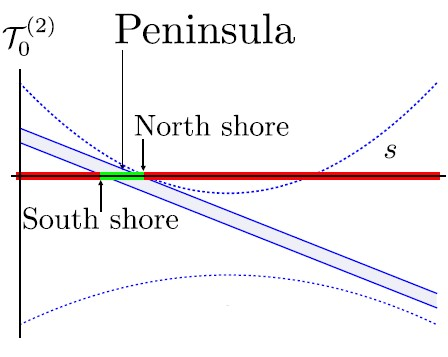
\includegraphics[width=6cm]{7.jpg}
  \caption{Penrose diagram for subextremal charged black hole}
  \label{fig:1}
\end{figure}
In subextremal black hole, the result of having two horizons is that if an object crosses the outer horizon from the outside or crosses the inner horizon from inside of it it has no choice but to travel to the other horizon. But an object falling into outer horizon after necessarily falling into the inner horizon can now escape by crossing the inner horizon which is possible since $t$ is now a timelike coordinate. This behaviour can be seen by looking at the Penrose diagram.

\section{Extremal Reissner-Nordstrom Black Hole}

\subsection{Metric Ansatz for Einstein Equations}
Putting $Q=M$, we get
$$
d s^{2}=-\left(1-\frac{M}{r}\right)^{2} d t^{2}+\left(\frac{1}{1-\frac{M}{r}}\right)^{2} d r^{2}+r^{2} d \Omega^{2}
$$
We want to describe multiple Extremal RNBHs. For that we prefer cartesian coordinates to spherical coordinates which are more appropriate for a single Extremal RNBH. To do this, we try to write the above as
$$
d s^{2}=-\left(1-\frac{M}{r}\right)^{2} d t^{2}+\left(\frac{1}{1-\frac{M}{r}}\right)^{2} \left(d r^{2}+(r-M)^{2} d \Omega^{2}\right)
$$
This suggests we write $\rho=r-M$ to get
$$
ds^{2}=-f(\rho)^{-2} d t^{2}+f(\rho)^{2}\left(d \rho^{2}+\rho^{2} d \Omega^{2}\right)=-f(\rho)^{-2} d t^{2}+f(\rho)^{2}\left(dx^{2}+dy^{2}+dz^{2}\right)
$$
where $f(\rho)=1+\frac{M}{\rho}$. Now while making the shift to multiple Extremal RNBHs, we lose spherical symmetry which makes $f(x,y,z)=f(\rho)$. So the ansatz we have for multiple Extremal RNBHs is given by
$$
d s^{2}=-f(x, y, z)^{-2} d t^{2}+f(x, y, z)^{2}\left(d x^{2}+d y^{2}+d z^{2}\right)
$$
\subsection{Vector Potential Ansatz for Maxwell's Equations}
We go back to a single BH to now look at electromagnetic field ansatz. For a single BH, the only nonzero component of $A_{\mu}$ is (keeping in mind $Q=M$ and the extra factor of $\sqrt{4 \pi}$ in $Q$,
$$A_{0}=\frac{Q}{\sqrt{4 \pi} r}=\frac{M}{\sqrt{4 \pi}(\rho+M)}=\frac{1-f(\rho)^{-1}}{\sqrt{4 \pi}}$$
which for the multiple case we write as 
$$
A_{0}=\frac{1}{\sqrt{4 \pi}}\left(1-f(x, y, z)^{-1}\right)
$$
NOTE:- This $f(x,y,z)$ is the same function as in the previous ansatz. There is no reason for this to be the case but we will check if doing this allows us to simultaneously solve both Einstein's and Maxwell's equations.

\subsection{Maxwell's Equation}
$$F_{0 i}=\partial_{0} A_{i}-\partial_{i} A_{0}=-\partial_{i} A_{0} =\frac{\partial_{i} f}{\sqrt{4 \pi}f^{2}},\quad F_{i j}=0$$
with $\partial_{i} \equiv \frac{\partial}{\partial x^{i}}$ and $\left(x^{1}, x^{2}, x^{3}\right)=(x, y, z)$ and using $\sqrt{-g}=f^{2}$ and the fact that $f$ is independent of $t$,
$$\frac{1}{\sqrt{-g}} \partial_{\mu}\left(\sqrt{-g} F^{\mu v}\right)=\frac{1}{\sqrt{-g}} \partial_{i}\left(\sqrt{-g} F^{i v}\right)=0 \Rightarrow \partial_{i}\left(f^{2} F_{0 i}\right)=0$$
$$ \Rightarrow  \nabla^{2} f=0$$

\subsection{Einstein's Equation}

\subsubsection{Energy Momentum Tensor}
$T_{\mu \nu}=F_{\mu \lambda} F_{\nu}^{\;\lambda}-\frac{1}{4} g_{\mu \nu} F_{\sigma \rho} F^{\sigma \rho}$ and since there is Cartesian symmetry we shall write down values corresponding to $x^{1}$ only to prevent confusion over repeated indices being thought of as summed over. $g_{00}=-1 / f^{2}, g_{11}=f^{2}, g^{00}=-f^{2}$, and $g^{11}=1 / f^{2}$.
$$F_{0 1} =\frac{\partial_{1} f}{\sqrt{4 \pi}f^{2}} \Rightarrow F^{01}=g^{00} g^{11} F_{01}=-\frac{\partial_{1} f}{\sqrt{4 \pi} f^{2}}$$
$$\Rightarrow F_{\sigma \rho} F^{\sigma \rho}=-2\frac{\left(\partial_{i} f\right)^{2}}{4 \pi f^{4}}$$
Using $F_{0}^{\;1}=g^{1 1} F_{0 1}=\frac{\partial_{1} f}{\sqrt{4 \pi} f^{4}}$,
$$T_{00}=F_{0 i} F_{0}^{\;i}-\frac{1}{4} g_{00} F_{\sigma \rho} F^{\sigma \rho}$$
$$
\Rightarrow 8 \pi T_{0 0}=\frac{\left(\partial_{i} f\right)^{2}}{f^{6}}
$$
Using $F_{1}^{\;0}=g^{0 0} F_{1 0}=\frac{\partial_{1} f}{\sqrt{4 \pi}}$,
$$T_{1 1}=F_{1 0} F_{1}^{\;0}-\frac{1}{4} g_{11} F_{\sigma \rho} F^{\sigma \rho}$$
$$
\Rightarrow 8 \pi T_{1 1}=\frac{\left(\partial_{i} f\right)^{2}-2\left(\partial_{1} f\right)^{2}}{f^{2}}
$$
$$T_{1 2}=F_{1 0} F_{2}^{\;0}$$$$\Rightarrow 8 \pi T_{1 2}=-\frac{2\left(\partial_{1} f\right)\left(\partial_{2} f\right)}{f^{2}}$$
And also its easy to see that $T_{0 i}=0$ and $T=g^{\mu \nu} T_{\mu \nu}=g^{0 0} T_{0 0} + 3 g^{1 1} T_{1 1}=0$.

\subsubsection{Ricci Tensor}
It is preferable to use Vielbins to calculate the Ricci tensor's components which turn out to be 
$$R_{00}=\frac{\left(\partial_{i} f\right)^{2}-f \nabla^{2} f}{f^{6}}, R_{11}=\frac{\left(\partial_{i} f\right)^{2}-2\left(\partial_{1} f\right)^{2}-f \nabla^{2} f}{f^{2}}, R_{12}=-\frac{2\left(\partial_{1} f\right)\left(\partial_{2} f\right)}{f^{2}}$$
Since energy momentum tensor is traceless, Einstein's equation is $R_{\mu \nu}=8 \pi T_{\mu \nu}$ and this leads to the same condition as the Maxwell's equation i.e.
$$
\nabla^{2} f(x, y, z)=0
$$
\subsection{Physical Explanation}
By demanding that $A_{0} \rightarrow 0$ far away to fix additive constant, we get
$$
\nabla^{2} f(x, y, z)=0 \Rightarrow f(\vec{x})=1+\sum_{a=1}^{N} \frac{M_{a}}{\left|\vec{x}-\vec{x}_{a}\right|}
$$
This is a time independent simultaneous solution of $N$ Extremal RNBHs sitting stationary at various locations.\\
The physical reason behind this is the fact that any Extremal RNBhs do not either attract or repel each other allows this situation to occur and the reason they don't attract or repel is that their repulsive Coulombic force $=\frac{Q_{a}Q_{b}}{4 \pi r}$ perfectly cancels the attractive Gravitational force $=\frac{M_{a}M_{b}}{4 \pi r}$ since Extremality $\Rightarrow Q_{a/b}=\sqrt{4 \pi}M_{a/b}$ which in hindsight makes looking for such a solution more hopeful.


\newpage











\appendix


\section{Computation of Ricci Tensor used in Sec 4.4.2}
We will be using Vielbin formalism to calculate Ricci tensor.\\
Step 1:- Write down vielbin $e$ from the metric using $ds^{2}=g_{\mu \nu}dx^{\mu}dx^{\nu}=\eta_{\alpha \beta}e^{\alpha}e^{\beta}$.\\
Step 2:- Use $de+ \omega e=0$ to extract $\omega$.\\
Step 3:- Use $R=d\omega + \omega^{2}$ to get Riemann tensor components.\\
Step 4:- Contract to get Ricci tensor components.\\


\subsection{Step 1}
A diagonal metric makes this trivial:
$e^{0}=f^{-1}(x,y,z)dt$, $e^{i}=f(x,y,z)dx^{i}$




\subsection{Step 2}
We have by diiferentiating, $de^{0}=-\dfrac{\partial_{i}f}{f^{2}}dx^{i}dt=\dfrac{\partial_{i}f}{f^{2}}dtdx^{i}$ \; and \; $de^{i}=(\partial_{j}f)dx^{j}dx^{i}$.\\
Rewriting them as $de^{0}+\left(-\dfrac{\partial_{i}f}{f^{3}}dt\right)(fdx^{i})=0 \Rightarrow de^{0}+\left(-\dfrac{\partial_{i}f}{f^{3}}dt+(...)dx^{i}\right)e^{i}=0$\\ 
Because since is no $dt$ term in $de^{i}$, the (...) has to be $0$ allowing us to write 
$$\omega^{0}_{\;i}=-\dfrac{\partial_{i}f}{f^{3}}dt=-\dfrac{\partial_{i}f}{f^{2}}e^{0}$$
And $de^{i}=(\partial_{j}f)dx^{j}dx^{i}$ means 
$$
\begin{array}{l}
d e^{1}=\left(\partial_{2} f\right) d x^{2} d x^{1}+\left(\partial_{3} f\right) d x^{3} d x^{1} \\
d e^{2}=\left(\partial_{3} f\right) d x^{3} d x^{2}+\left(\partial_{1} f\right) d x^{1} d x^{2} \\
d e^{3}=\left(\partial_{1} f\right) d x^{1} d x^{3}+\left(\partial_{2} f\right) d x^{2} d x^{3} 
\end{array}
$$
We get
$\omega_{\;\;2}^{1}=\frac{\partial_{2} f}{f} d x^{1}+(\cdots) d x^{2}$ and $\omega^{2}_{\;\;1}=-\omega^{1}_{\;\;2}=\frac{\partial_{1} f}{f} d x^{2}+(\cdots) d x^{1}$ which combine to give
$$\omega_{\;\;2}^{1}=\frac{\partial_{2} f}{f} d x^{1}-\frac{\partial_{1} f}{f} d x^{2}$$ 
and in general 
$$\omega_{\;\;j}^{i}=\frac{\partial_{j} f}{f} d x^{i}-\frac{\partial_{i} f}{f} d x^{j}=\frac{\partial_{j} f}{f^{2}} e^{i}-\frac{\partial_{i} f}{f^{2}} e^{j}$$ 





\subsection{Step 3 and 4}
Differentiating $\omega^{0}_{\;i}=-\dfrac{\partial_{i}f}{f^{3}}dt$ gives
$$
d \omega^{0}_{\;\;i}=\frac{3\left(\partial_{i} f\right)\left(\partial_{j} f\right)}{f^{4}}  d x^{j} d t -\frac{\partial_{j} \partial_{i} f}{f^{3}} d x^{j} d t
$$
$$
\Rightarrow d \omega^{0}_{\;\;i}=\frac{f\partial_{j} \partial_{i} f -3\left(\partial_{i} f\right)\left(\partial_{j} f\right)}{f^{4}} e^{0}e^{j}
$$
Differentiating $\omega_{\;\;j}^{i}$ gives
$$
d \omega^{i}_{j}= \frac{\partial_{k} \partial_{j} f}{f} d x^{k} d x^{i}-\frac{(\partial_{j} f)\left(\partial_{k} f\right)}{f^{2}} d x^{k} d x^{i} -\frac{\partial_{k} \partial_{i} f}{f} d x^{k} d x^{j}+\frac{\left(\partial_{i} f\right)\left(\partial_{k} f\right)}{f^{2}} d x^{k} d x^{j}
$$
$$
\Rightarrow d \omega^{i}_{\;\;j}= \frac{(\partial_{j} f)\left(\partial_{k} f\right)-f\partial_{k} \partial_{j} f}{f^{4}}e^{i} e^{k} +\frac{f\partial_{k} \partial_{i} f-\left(\partial_{i} f\right)\left(\partial_{k} f\right)}{f^{4}} e^{j} e^{k}
$$
Now to calculate $\omega^{2}$ part,
$$
\omega_{\;\;\alpha}^{0} \omega^{\alpha}_{\;\;i}=\omega^{0}_{ \;\;0} \omega^{0}_{\;\;j} +\omega^{0}_{\;\;k} \omega^{k}_{\;\;i}=\omega^{0}_{\;\;j} \omega^{j}_{\;\;i}=\left(-\dfrac{\partial_{j}f}{f^{2}}e^{0} \right) \left(\frac{\partial_{i} f}{f^{2}} e^{j}-\frac{\partial_{j} f}{f^{2}} e^{i} \right)
$$
$$
R_{\;\;i}^{0}=d \omega^{0}_{\;\;i}+\omega_{\;\;\alpha}^{0} \omega^{\alpha}_{\;\;i}=\frac{f\partial_{j} \partial_{i} f -4\left(\partial_{i} f\right)\left(\partial_{j} f\right)}{f^{4}} e^{0}e^{j}+\frac{\left(\partial_{j}f \right)^{2}}{f^{4}}e^{0}e^{i}
$$
$$
\Rightarrow R_{\;\;1}^{0}=\frac{f\partial_{j} \partial_{1} f -4\left(\partial_{1} f\right)\left(\partial_{j} f\right)}{f^{4}} e^{0}e^{j}+\frac{\left(\partial_{j}f \right)^{2}}{f^{4}}e^{0}e^{1}
$$
$R_{\;\;1 0 1}^{0}$ is coefficient of $e^{0}e^{1}$ in $R_{\;\;1}^{0}$,
$$
\Rightarrow R_{\;\;1 0 1}^{0}=\frac{f\partial_{1}^{2} f -4\left(\partial_{1} f\right)^{2}+\left(\partial_{i} f\right)^{2}}{f^{4}} 
$$
$$
\Rightarrow R_{\;\;0}^{0}=\sum_{j=1}^{3} R_{\;\;j 0 j}^{0}=\frac{f \nabla^{2} f-4\left(\partial_{i} f\right)^{2}+3\left(\partial_{i} f\right)^{2}}{f^{4}}=\frac{f \nabla^{2} f-\left(\partial_{i} f\right)^{2}}{f^{4}}
$$
$$
\Rightarrow R_{tt}=e_{t}^{\mu} e_{t}^{\nu} \eta_{\mu \rho} R^{\rho}_{\;\;\nu}=e_{t}^{0} e_{t}^{0} \eta_{00} R^{0}_{\;\;0}=-\frac{1}{f^{2}} R^{0}_{\;\;0}=\frac{\left(\partial_{i} f\right)^{2}-f \nabla^{2} f}{f^{6}}
$$
$$
\Rightarrow R_{tt}=\frac{\left(\partial_{i} f\right)^{2}-f \nabla^{2} f}{f^{6}}
$$
Now moving on to $\omega_{\;\;\alpha}^{i} \omega^{\alpha}_{\;\;j}$,
$$
\omega_{\;\;\alpha}^{i} \omega^{\alpha}_{\;\;j}=\omega^{i}_{ \;\;0} \omega^{0}_{\;\;j} +\omega^{i}_{\;\;k} \omega^{k}_{\;\;j}
$$
We know that both $\omega^{i}_{ \;\;0}$,$\omega^{0}_{\;\;j} \propto dt$ and hence that term is zero.
$$\omega^{i}_{\;\;k} \omega^{k}_{\;\;j}=\left( \frac{\partial_{k} f}{f^{2}} e^{i}-\frac{\partial_{i} f}{f^{2}} e^{k}\right)\left( \frac{\partial_{j} f}{f^{2}} e^{k}-\frac{\partial_{k} f}{f^{2}} e^{j}\right)$$
Although complicated looking we see this contributes only if $i\neq k$ and $j\neq k$ and since there are just 3 coordinates, we have just one $k$ contributing. So we have 
$$
\begin{aligned}
R_{\;\;2}^{1}&=d \omega_{\;\;2}^{1}+\omega_{\;\;3}^{1} \omega^{3}_{\;\;2}\\
&=d\left[\frac{\left(\partial_{2} f\right) d x^{1}-\left(\partial_{1} f\right) d x^{2}}{f}\right]+\left[\frac{\left(\partial_{3} f\right) d x^{1}-\left(\partial_{1} f\right) d x^{3}}{f}\right]\left[\frac{\left(\partial_{2} f\right) d x^{3}-\left(\partial_{3} f\right) d x^{2}}{f}\right]
\end{aligned}
$$
$$
\begin{array}{r}
R_{\;\;2}^{1}=\dfrac{1}{f^{2}}[-(\partial_{2} f)^{2} d x^{2} d x^{1} -\left(\partial_{2} f\right)\left(\partial_{3} f\right) d x^{3} d x^{1} +(\partial_{1} f)^{2} d x^{1} d x^{2}+\left(\partial_{1} f\right)\left(\partial_{3} f\right) d x^{3} d x^{2} \\\\
+\left(\partial_{3} f\right)\left(\partial_{2} f\right) d x^{1} d x^{3}+\left(\partial_{1} f\right)\left(\partial_{3} f\right) d x^{3} d x^{2}-(\partial_{3} f)^{2} d x^{1} d x^{2}+f\left(\partial_{2} \partial_{2} f\right) d x^{2} d x^{1}\\\\
+f\left(\partial_{3} \partial_{2} f\right) d x^{3} d x^{1}-f\left(\partial_{1} \partial_{1} f\right) d x^{1} d x^{2}-f\left(\partial_{1} \partial_{3} f\right) d x^{3} d x^{2}]
\end{array}
$$
and we have $dx^{i}dx^{j}=\dfrac{e^{i}e^{j}}{f^{2}}$ and using reindexing and symmetry of Ricci tensor (the lowering and raising of indices using Minkowski tensor to be kept in mind) we can get all components of Riemann tensor. By looking at coefficient of $e^{1}e^{2}$,we have
$$
R_{\;\;212}^{1}=R_{\;\;121}^{2}=\frac{1}{f^{4}}\left[\left(\partial_{j} f\right)^{2}-2\left(\partial_{3} f\right)^{2}-f \nabla^{2} f+f\left(\partial_{3} \partial_{3} f\right)\right]
$$
$$
R_{\;\;131}^{3}=\frac{1}{f^{4}}\left[\left(\partial_{j} f\right)^{2}-2\left(\partial_{2} f\right)^{2}-f \nabla^{2} f+f\left(\partial_{2} \partial_{2} f\right)\right]
$$
From earlier calculations, we have
$$
R_{\;\;101}^{0}=\frac{f \partial_{1}^{2} f-4\left(\partial_{1} f\right)^{2}+\left(\partial_{i} f\right)^{2}}{f^{4}}
$$
Adding the 3 up,
$$
R_{11}=\frac{\left(\partial_{j} f\right)^{2}-2\left(\partial_{1} f\right)^{2}-f \nabla^{2} f}{f^{4}}
$$
$$
R_{xx}=e^{1}_{x}e^{1}_{x}R_{11}=\frac{\left(\partial_{j} f\right)^{2}-2\left(\partial_{1} f\right)^{2}-f \nabla^{2} f}{f^{2}}
$$
$$
R_{12}=R_{\;\;102}^{0}+R_{\;\;132}^{3}=R_{\;\;102}^{0}+R_{\;\;323}^{1}
$$
$$
R_{\;\;1}^{0}=\frac{f \partial_{j} \partial_{1} f-4\left(\partial_{1} f\right)\left(\partial_{j} f\right)}{f^{4}} e^{0} e^{j}+\frac{\left(\partial_{j} f\right)^{2}}{f^{4}} e^{0} e^{1}\Rightarrow R_{\;\;102}^{0}=\frac{f \partial_{2} \partial_{1} f-4\left(\partial_{1} f\right)\left(\partial_{2} f\right)}{f^{4}}
$$
One can replace $2$ with $3$ in $R_{\;\;2}^{1}$ to get $R_{\;\;3}^{1}$ and extract coefficient of $e^{2}e^{3}$ to get 
$$
R_{\;\;323}^{1}=\frac{2\left(\partial_{1} f\right)\left(\partial_{2} f\right)-f \partial_{2} \partial_{1} f}{f^{4}}
$$
$$
R_{12}=-2\frac{\left(\partial_{1} f\right)\left(\partial_{2} f\right)}{f^{4}}
$$
$$
R_{xy}=e^{1}_{x}e^{2}_{y}R_{12}=-2\frac{\left(\partial_{1} f\right)\left(\partial_{2} f\right)}{f^{2}}
$$


\section{Black Hole solutions to Einstein's Field Equations}

\subsection{Getting to Schwarzschild Solution}

For a spherically symmetric metric given by
$$d s ^ { 2 } = - A ( r ) d t ^ { 2 } + B ( r ) d r ^ { 2 } + r ^ { 2 } d \Omega ^ { 2 }$$
or
$$g _ { t t } = - A ( r ) , \quad g _ { r r } = B ( r ) , \quad g _ { \theta \theta } = r ^ { 2 } , \quad g _ { \varphi \varphi } = r ^ { 2 } \sin ^ { 2 } \theta$$
We can extract Christoffel symbols by varying the Lagrangian
$$L = \left[ A ( r ) \left( \frac { d t } { d \tau } \right) ^ { 2 } - B ( r ) \left( \frac { d r } { d \tau } \right) ^ { 2 } - r ^ { 2 } \left( \frac { d \theta } { d \tau } \right) ^ { 2 } - r ^ { 2 } \sin ^ { 2 } \theta \left( \frac { d \varphi } { d \tau } \right) ^ { 2 } \right] ^ { \frac { 1 } { 2 } }$$
By varying, we get the four equations
$$\frac { d } { d \tau } \left( A ( r ) \frac { d t } { d \tau } \right) = 0 $$
$$\frac { d } { d \tau } \left( B ( r ) \frac { d r } { d \tau } \right) + \frac { 1 } { 2 } A ^ { \prime } ( r ) \left( \frac { d t } { d \tau } \right) ^ { 2 } - \frac { 1 } { 2 } B ^ { \prime } ( r ) \left( \frac { d r } { d \tau } \right) ^ { 2 } - r \left( \frac { d \theta } { d \tau } \right) ^ { 2 } - r \sin ^ { 2 } \theta \left( \frac { d \varphi } { d \tau } \right) ^ { 2 } = 0$$
$$\frac { d } { d \tau } \left( r ^ { 2 } \frac { d \theta } { d \tau } \right) - r ^ { 2 } \sin \theta \cos \theta \left( \frac { d \varphi } { d \tau } \right) ^ { 2 } = 0$$
$$\frac { d } { d \tau } \left( r ^ { 2 } \sin ^ { 2 } \theta \frac { d \varphi } { d \tau } \right) = 0$$
These are precisely the equations contained in the geodesic equation for the spherically symmetric metric.\\ \\
And we have defining equation for $\tau $
$$A ( r ) \left( \frac { d t } { d \tau } \right) ^ { 2 } - B ( r ) \left( \frac { d r } { d \tau } \right) ^ { 2 } - r ^ { 2 } \left( \frac { d \theta } { d \tau } \right) ^ { 2 } - r ^ { 2 } \sin ^ { 2 } \theta \left( \frac { d \varphi } { d \tau } \right) ^ { 2 } = 1$$
This equation can be used instead of the third equation among the four above and will have a $0$ instead of $1$ in $R.H.S$ in case of massless particles.\\
We now by comparision with geodesic equation have the Christoffel symbols given by
$$\begin{aligned} \Gamma _ { t r } ^ { t } & = \frac { A' } { 2 A } , \quad \Gamma _ { t t } ^ { r } = \frac { A' } { 2 B } , \quad \Gamma _ { r r } ^ { r } =  \frac { B' } { 2 B } , \quad \Gamma _ { \theta \theta } ^ { r } = - \frac { r } { B } , \quad \Gamma _ { \varphi \varphi } ^ { r } = - \frac { r \sin ^ { 2 } \theta } { B } \\ \Gamma _ { r \theta } ^ { \theta } & = \frac { 1 } { r } , \quad \Gamma _ { r \varphi } ^ { \varphi } = \frac { 1 } { r }\\  \Gamma _ { \varphi \varphi } ^ { \theta } & = - \sin \theta \cos \theta , \quad \Gamma _ { \theta \varphi } ^ { \varphi } = \cot \theta \end{aligned}$$
As of now, we only know that far away from the mass,
$A ( r ) \simeq \left( 1 - \frac { 2 G M } { r } \right)$ as $r \rightarrow \infty ,$ so that we recover the Newtonian gravitational potential
$\Phi ( r ) = - \frac { G M } { r } .$ To determine $A ( r )$ and $B ( r ) ,$ we would need to use the Einstein Field Equations.\\ \\
In empty spacetime (around a star or a black hole for example) the Ricci tensor vanishes.
$$R _ { \mu \nu } = 0$$
We need to compute the Riemann curvature tensor and thence the Ricci tensor. Then determine the two unknown functions $A$ and $B$ by solving Einstein's equation with the boundary condition $A ( r ) \rightarrow \left( 1 - \frac { 2 G M } { r } \right)$ and $B ( r ) \rightarrow 1$ as $r \rightarrow \infty .$\\ \\
Using
$$R _ { \nu \rho } = \left( \partial _ { \sigma } \Gamma _ { \nu \rho } ^ { \sigma } + \Gamma _ { \sigma \kappa } ^ { \sigma } \Gamma _ { \nu \rho } ^ { \kappa } \right) - \left( \partial _ { \nu } \Gamma _ { \sigma \rho } ^ { \sigma } + \Gamma _ { \nu \kappa } ^ { \sigma } \Gamma _ { \sigma \rho } ^ { \kappa } \right)$$
we obtain
$$\begin{aligned} R _ { t t } & = \frac { A ^ { \prime \prime } } { 2 B } + \frac { A ^ { \prime } } { r B } - \frac { A ^ { \prime } } { 4 B } \left( \frac { A ^ { \prime } } { A } + \frac { B ^ { \prime } } { B } \right) \\ R _ { r r } & = - \frac { A ^ { \prime \prime } } { 2 A } + \frac { B ^ { \prime } } { r B } + \frac { A ^ { \prime } } { 4 A } \left( \frac { A ^ { \prime } } { A } + \frac { B ^ { \prime } } { B } \right) \\ R _ { \theta \theta } & = 1 - \frac { 1 } { B } - \frac { r } { 2 B } \left( \frac { A ^ { \prime } } { A } - \frac { B ^ { \prime } } { B } \right)  \\ R _ { \varphi \varphi } & = \sin ^ { 2 } \theta R _ { \theta \theta } \end{aligned}$$
and all other components vanishing.\\ \\
Using the first two we get
$$\frac { R _ { t t } } { A } + \frac { R _ { r r } } { B } = \frac { 1 } { r B } \left( \frac { A ^ { \prime } } { A } + \frac { B ^ { \prime } } { B } \right) = 0 .$$
This instantly solves itself as $A B = 1$ where we fixed the integration constant by the boundary condition at $r \rightarrow \infty.$\\ \\ 
Eliminating $\frac { A ^ { \prime } } { A } = - \frac { B ^ { \prime } } { B }$ the third equation, we get 
$$r \left( \frac { 1 } { B } \right) ^ { \prime } + \frac { 1 } { B } = 1$$
with solution
$$\frac { 1 } { B } = 1 + \frac { b } { r }$$
So,
$$A = 1 + \frac { b } { r }$$
The boundary condition at infinity fixes the integration constant $b$ to be $- 2 G M$.
We hence arrive at the Schwarzschild Metric
$$d s ^ { 2 } = - \left( 1 - \frac { 2 G M } { r } \right) d t ^ { 2 } + \frac { 1 } { \left( 1 - \dfrac { 2 G M } { r } \right) } d r ^ { 2 } + r ^ { 2 } \left( d \theta ^ { 2 } + \sin ^ { 2 } \theta d \varphi ^ { 2 } \right)$$

\subsection{Coordinate vs Physical Singularity}
The singularity at $r _ { \mathrm { S } } \equiv 2 G M$ is a coordinate singularity. The scalar quantity $R ^ { \mu \nu \rho \sigma } R _ { \mu \nu \rho \sigma }$ is equal to $\dfrac { 12 r _ { \mathrm { S } } ^ { 2 } } { r ^ { 6 } }$ which has no peculiar behaviour at $r = r _ { \mathrm { S } }$. However, there is a real physical singularity at $r = 0$ and the scalar $R ^ { \mu \nu \rho \sigma } R _ { \mu \nu \rho \sigma }$ blows up at $r = 0$ as a result. 

\subsection{Black Hole}
The Schwarzschild solution holds only for $r > R$ since the Ricci tensor vanishes in free space and so it holds only outside the body which is the source of the gravitational field. The Schwarzschild radius of an ordinary massive object, the sun for example, is much less than its characteristic size $R$ and so would be located inside the object, where the Schwarzschild solution is not relevant. This is the case for all objects except black holes. Black holes are so compact that $r=r_{s}$ is empty space and hence Schwarschild solution is valid and there $g_{00} \rightarrow 0$ i.e there is infinite redshift and below that radius not even light can escape. Hence no information about any event inside the Schwarschild radius can escape to the outside world and hence the coordinate singularity is called an Event Horizon.







\newpage
\textbf{References}\\\\
1. Einstein Gravity in a Nutshull by Anthony Zee\\
2. Gravitation: Foundation and Frontiers by Thanu Padmanabhan\\
3. Gravitation and Cosmology by Weinberg\\
4. Introduction to the Theory of Black Holes by Gerard ’t Hooft\\
5. Lectures on General Theory of Relativity by ET Akhmedov
\\ \\



\end{document}

